 A basic event selection is made for selecting signal like events. The necessary event requirement are discussed in \Sec{sec:selection}. 

The analysis uses signal and background regions to constrain the huge \SM\ background compared to the expected signal. \Sec{sec:regions} discusses each region that is entering the analysis. On top of the use of background estimation from control regions, backgrounds that have  prompt leptons  contaminated by real leptons either
from decays of tau leptons or from hadronized mesons or baryons
(collectively commonly referred as ``non-prompt leptons") as well as by
hadrons or jets misidentified as leptons\footnote{These two classes
	of contamination will be referred to as not prompt-lepton (\NPL) samples.} are
evaluated with a data-driven method discussed in \Sec{sec:NPL}.


\section{Baseline event selection and filters}
The CMS collaboration recorded in the course of 2016 proton at 13 \TeV\ collisions data  with a total recorded integrated luminosity of $35.9 \pm 2.5\%~\fbinv$. The baseline event selection has a goal to substantially reject SM background events, whilst maintaining a high signal efficiency. In this analysis a search is performed in a final state made up of a \PZ\ boson and a top quark, associated or not with a jet, in the leptonic decay of the \PZ\ boson and the top quark. The leading order Feynman diagrams can be seen in Figure \ref{fig:Feynmanlep}\todo{adapt to leptonic decay}.  
\begin{figure}[hbtp]
	\centering
	\subbottom[]{
		\begin{fmffile}{singletoplep}
			\begin{fmfgraph*}(160,40) % width - height
				\fmfleft{i1,i2} 
				\fmfright{o1,o2}
				\fmf{fermion}{i1,v1,v2,o2}
				\fmf{boson}{v2,o1}
				\fmf{gluon}{i2,v1}
				\fmflabel{\Pgluon}{i2}
				\fmflabel{\Pup,\Pcharm}{i1}
				\fmfv{label= ,decor.shape=circle,decor.filled=shaded,decor,size=0.5thick, label.angle=-90}{v2}
				% \fmflabel{\Pup,\Pcharm}{i1}
				\fmflabel{\PZ}{o1}
				\fmflabel{\Ptop}{o2}
				\fmf{fermion,label=\Pup,,\Pcharm,label.dist=10}{v1,v2}
			\end{fmfgraph*}
		\end{fmffile}
	}
	\hspace*{1cm}
	\subbottom[]{
		\begin{fmffile}{toppairlep}
			\begin{fmfgraph*}(160,40) % width - height
				\fmfleft{i1,i2} 
				\fmfright{o1,o2,o3,o4}
				\fmflabel{\Pgluon}{i1}
				\fmflabel{\Pgluon}{i2}
				\fmflabel{\APup,\APcharm}{o1}
				\fmflabel{\PZ}{o2}
				\fmflabel{\PWp}{o3}
				\fmflabel{\Pbottom}{o4}
				\fmf{gluon}{i1,v1,i2}
				\fmf{gluon,label=\Pgluon,label.dist=10}{v1,v2}
				\fmf{fermion}{o1,v4,v2,v3,o4}
				\fmffreeze
				\fmf{boson}{v3,o3}
				\fmf{boson}{v4,o2}
				\fmfv{label= ,decor.shape=circle,decor.filled=shaded,decor,size=0.2thick, label.angle=-90}{v4}
				\fmf{fermion,label=\Ptop,label.dist=5}{v2,v3}
				\fmf{fermion,label=\APtop,label.dist=-20}{v4,v2}
				\fmflabel{}{v3}
				\fmflabel{}{v2}
				\fmflabel{}{v1}
			\end{fmfgraph*}
		\end{fmffile}
	}
	\caption{Feynman diagrams for the \tZq\ \FCNC\ interaction with a fully leptonic decay, where the FCNC interaction is indicated with the shaded dot. (a) Single top production through an \FCNC\ interaction. (b) Top pair production with an \FCNC\ induced decay. }
	\label{fig:Feynmanlep}
\end{figure}

The signal considers both the single top \FCNC\ (\tZ\ in the final state) and the top pair \FCNC\ (\tZq\ in the final state) events. Their final state signatures consist of three leptons, considering electrons or muons in our analysis, and a jet originating from a b quark. For \FCNC\ \tZq, there is an additional up or charm jet. Leptons from tau decays are not vetoed and are entering the analysis. Four different lepton channels based on lepton flavour are considered (\eee, \eemu, \emumu, and \mumumu).  


The CMS trigger system, described in \Sec{sec:DAQ}, filters out the main of the collision events from uninteresting processes and dedicated trigger paths are define to single out the events with our required detector signature. The trigger paths are chosen based on on-line triggering objects with at least one muon (M), at least one electron (E), at least two muons (MM), at least two electrons (EE), at least one muon and an electron (ME), at least three muons (MMM), at least three electrons (EEE), at least two muons and one electron (MME), or at least two electrons and one muon (EEM). For the MC simulation a simple $or$ of all triggers is taken and the event is taken if it passes one of the trigger paths. For data however, double counting of the same event has to be taken into account and a procedure to avoid double counting has been put into place. It consists of vetoing in a given dataset the events that are already selected in another, as given in Table \ref{tab:triggerlogic}. 
\begin{table}[htbp]
	\centering
	\caption{Trigger logic used to select data events in order to avoid double counting}
	\begin{tabular}{ll}
		\toprule
		Dataset & Trigger Logic \\ 
		\midrule
		\emu & EM $\Arrowvert$ EEM $\Arrowvert$ MME \\ 
		
		\mumu & (MM $\Arrowvert$ MMM) \&\& !( EM $\Arrowvert$ EEM $\Arrowvert$ MME)  \\ 
		
		\ee & (EE $\Arrowvert$ EEE) \&\& !(MM $\Arrowvert$ MMM) \&\& !( EM $\Arrowvert$ EEM $\Arrowvert$ MME) \\ 
		
		single \Pmu & M \&\& !(EE $\Arrowvert$ EEE) \&\& !(MM $\Arrowvert$ MMM) \&\& !( EM $\Arrowvert$ EEM $\Arrowvert$ MME) \\ 
		
		single e & E \&\& !M \&\& !(EE $\Arrowvert$ EEE) \&\& !(MM $\Arrowvert$ MMM) \&\& !( EM $\Arrowvert$ EEM $\Arrowvert$ MME)  \\ 
		\bottomrule
	\end{tabular} 
	\label{tab:triggerlogic}
\end{table}

This trigger selection strategy is to allow the maximum statistics on the signal region since it does not  discard events from any dataset.  For the single lepton triggers, at least one electron (muon) with a transverse momentum \pt higher than 32~\GeV\ (24~\GeV) is required.  The dilepton triggers require an electron (muon) with $\pt > 23~\GeV$ and a muon (electron) with $\pt > 8~\GeV$, or an electron (muon) with $\pt > 23~\GeV$ (17~\GeV) and an electron (muon) with $\pt > 12~\GeV$ (8~\GeV). Events collected by the trilepton triggers require  an electron (muon) with $\pt > 16~\GeV$ (12~\GeV), a second electron (muon) of  $\pt > 12~\GeV$ (10~\GeV),  and a third electron (muon) with $\pt > 8~\GeV$ (5~\GeV). The mixed trilepton trigger events require two electrons (muons) with $\pt > 12~\GeV$ (9~\GeV)  and a third muon (electron) with $\pt > 8~\GeV$ (9~\GeV). The HLT trigger paths used in data and simulation are summarised in \tab{tab:Trigger}. 
\begin{table}[h]
	\centering
	\caption{HLT trigger paths used to select data and simulation events.}
	\begin{tabular}{lc}
		\toprule
		Trigger path name &  Trigger type \\ 
		\midrule
		HLT\_Mu23\_TrkIsoVVL\_Ele8\_CaloIdL\_TrackIdL\_IsoVL\_v &  ME \\ 
		%		\hline 
		HLT\_Mu23\_TrkIsoVVL\_Ele8\_CaloIdL\_TrackIdL\_IsoVL\_DZ\_v &  ME \\ 
		%		\hline 
		HLT\_Mu8\_TrkIsoVVL\_Ele23\_CaloIdL\_TrackIdL\_IsoVL\_v &  ME \\ 
		%		\hline 
		HLT\_Mu8\_TrkIsoVVL\_Ele23\_CaloIdL\_TrackIdL\_IsoVL\_DZ\_v &  ME \\ 
		%		\hline 
		HLT\_DiMu9\_Ele9\_CaloIdL\_TrackIdL\_v &  MME \\ 
		%		\hline 
		HLT\_Mu8\_DiEle12\_CaloIdL\_TrackIdL\_v &  EEM \\ 
		\midrule
		HLT\_IsoMu24\_v &  M \\ 
		%		\hline 
		HLT\_IsoTkMu24\_v &  M \\ 
		\midrule
		HLT\_Ele32\_eta2p1\_WPTight\_Gsf\_v &  E \\ 
		\midrule
		HLT\_Mu17\_TrkIsoVVL\_Mu8\_TrkIsoVVL\_v &  MM \\ 
		%		\hline 
		HLT\_Mu17\_TrkIsoVVL\_TkMu8\_TrkIsoVVL\_v &  MM \\ 
		%		\hline 
		HLT\_Mu17\_TrkIsoVVL\_Mu8\_TrkIsoVVL\_DZ\_v &  MM \\ 
		%		\hline 
		HLT\_Mu17\_TrkIsoVVL\_TkMu8\_TrkIsoVVL\_DZ\_v &  MM \\ 
		%		\hline 
		HLT\_TripleMu\_12\_10\_5\_v &  MMM \\ 
		\midrule
		HLT\_Ele23\_Ele12\_CaloIdL\_TrackIdL\_IsoVL\_DZ\_v &  EE \\ 
		HLT\_Ele16\_Ele12\_Ele8\_CaloIdL\_TrackIdL\_v &  EEE \\ 
		\bottomrule 
	\end{tabular} 
	\label{tab:Trigger}
\end{table}

In order to ensure a full trigger efficiency, the offline \pt\ treshodls are siet higher than the on-lon etrigger thresholds. 
Selected electrons (muons) are required to have \pt $>$ 35 (30)~\GeV\ and $|\eta| < 2.1 (2.4)$. A quantity for evaluating lepton isolation is calculated as the summed energy of all particles (charged hadrons, neutral hadrons, photons) in a cone of radius $\Delta R < 0.3 \;(0.4)$ around the electron (muon), excluding the electron (muon) itself, and divided by the lepton \pt.  An electron candidate is selected if this isolation quantity is below 0.059 in the barrel region and below 0.057 in the end caps.  A muon candidate is selected if this isolation quantity is below 0.15. Other lepton selection criteria are applied in analysis based on the values of various quantities determined during the reconstruction, such as number of missing track hits or the electromagnetic shower created by the particles. These are given in \Sec{sec:MuonID} (\tab{tab:MuonReq}) and \Sec{sec:ElectronID} (\tab{tab:ElecReq}). The trigger efficiency estimation is described in Section \ref{sec:triggereff}.


The samples are pre-selected off-line to ensure that all reconstructed particles considered for the analysis are corresponding to a proton interaction and that signals from beam halo particles as well as detector noise is removed. For this reason, several filters are used. These are described in \Sec{sec:Filters}.

On top of leptons, jets and missing transverse energy are expected from the signal signature. The jets are reconstructed using the \antikt\ algorithm with a distance parameter of 0.4 using the particle flow particles that are not identified as isolated leptons as input. The jet momentum is determined as the vectorial sum of the particles contained in the jet. Additional selection criteria are applied to each event to remove spurious jet-like features originating from isolated noise patterns in certain hadron calorimeter regions. More information about the jets used for this analysis can be found in \Sec{sec:JetID}. The jets are calibrated in simulation and in data separately, accounting for deposits from \pu\ and the non-linear detector response. Calibrated jets with \pt $> 30$~\GeV\ and $|\eta| < 2.4$ are selected.  A selected jet may still overlap with the selected leptons leading to a double-counting. To prevent such cases, jets that are found within a cone of  $R = 0.3$ around any of the signal electrons (muons) are removed from the set of selected jets.

The jets originating from b quarks are tagged using the CSVv2 algorithm, which combines the information of displaced tracks with information of secondary vertices associated with the jet using a multivariate technique. The jets are tagged as a jet coming from a b quark (b-tagged) if the CSVv2 discriminator is above a certain threshold.  This analysis uses a threshold that results in an average b-tagging efficiency of 81\% and a misidentification rate of 10\%. More information about b-tagging can be found in \Sec{sec:BJetID}.

The missing transverse momentum vector \ptmisvec\ is defined as the projection on the plane perpendicular to the beams of the negative vector sum of the momenta of all reconstructed particles in an event. Its magnitude is denoted by \Etmis as shown in \Sec{sec:MET}. Its longitudinal component is calculated by limiting the lepton + neutrino to the \PW\ boson mass. In case two solutions arise, the mass closest to the known top quark mass is used. 
The events and their corresponding object collections reconstructed using the reconstruction criteria described in Section \ref{sec:reco}, are used as input for the analysis. Further requirements on the momenta and the pseudo rapidities are made to fulfil the trigger requirements and reconstruction algorithms. %These are given in Table \ref{tab:pteta}.
%\begin{table}[h]
%	\centering
%	\caption{Momentum and pseudo rapidity requirements on the reconstructed objects.}
%	\begin{tabular}{c|c|c}
%		\hline 
%		& \pt$>$ & $|\eta|<$ \\ 
%		\hline 
%		muons & 30 \GeV & 2.4 \\ 
%		\hline 
%		electrons & 35 \GeV & 2.1 \\ 
%		\hline 
%		jets & 30 \GeV & 2.4 \\ 
%		\hline 
%	\end{tabular} 
%	\label{tab:pteta}
%\end{table}
\subsection{Event cleaning}
\label{sec:Filters}
REWRITE %%met filter %http://cds.cern.ch/record/2205284/files/JME-16-004-pas.pdf

Some events arising from instrumental noise and beam backgrounds might end up in the data. By use of filters, such non collision events are omitted~\cite{Filters}. 
\begin{description}
	\item [Beam halo] The machine induced particles, via beam-gas / beam-pipe/... interactions, that are flying with the beam affect the physics analysis. Therefore, events containing such beam halo particles are removed from the selection with the CSC Beam Halo Filter. 
	\item [HBHE nois] The HB and HE are known to record sporadic anomalous signals (noise) at a fixed rate independent of the beam conditions. The events are cleaned for this noise by use of algorithms that exploit the geometrical patterns and pulse shape information of the known noise. 
	\item 	[ee badSC noise]  There are two supercrystal regions that give anomalous high energies and events suffering from this problem have to be removed. This affects only data and is therefore not applied on simulation. 
	\item [ECAL TP] The ECAL dead cell trigger primitive filter is used to correct for channels where the primary data links were down during data taking. It also corrects for ECAL noisy crystals that were masked during the reconstruction of the event. 
	\item [Bad Muons] There is a reconstruction issue leading to high \pt\ muons at $\abs{\eta}>2.3$. This causes artificial multi-\TeV\ tails in the distribution of the missing transverse energy for both MC and data. If the muons are low quality, they will be mislabelled as charged hadrons. By investigation the compatibility between non particle flow muon candidates and particle flow charged hadrons, these events can be filtered out. 
\end{description}

% see https://indico.cern.ch/event/591506/contributions/2387636/attachments/1381281/2099935/2016_12_01_MET_Scanning_Report_PPD.pdf
% see https://indico.cern.ch/event/537458/contributions/2184619/attachments/1281045/1903148/met_scanner_report_may30.pdf
% see https://indico.cern.ch/event/534040/contributions/2178680/attachments/1280427/1901837/HCALnoise_JamboreeMeeting_27May2016.pdf
%see https://indico.cern.ch/event/518559/contributions/2132815/attachments/1264581/1871184/beamhalostatus.pdf
% see https://twiki.cern.ch/twiki/bin/viewauth/CMS/MissingETOptionalFiltersRun2

Additionally, only events with where the first primary vertex is a well reconstructed primary vertex are selected. The reconstructed primary vertex should have at least five degrees of freedom, the longitudinal distance from the beam spot is maximally 24 cm ($d_z < 24$ cm), and the transversal distance from the beam spot is maximally 2 cm ($d_{xy}<2$ cm ). 
\subsection{Estimation of the trigger efficiency}
\label{sec:triggereff}
The trigger efficiency in data is estimated using a data sample collected using unprescaled MET triggers, following the approach of \cite{CMSAN2016276}. The events passing the trigger paths:
\begin{itemize}
	\item HLT\_PFHT300\_PFMET110\_v*, or
	\item HLT\_MET200\_v*, or 
	\item HLT\_PFMET300\_v*, or
	\item HLT\_PFMET120\_PFMHT120\_IDTight\_v*, or
	\item HLT\_PFMET170\_HBHECleaned\_v*
\end{itemize}
are being considered for the test data sample. These trigger paths are chosen to be completely uncorrelated with the lepton triggers given in Table \ref{tab:Trigger}. The studied simulation sample is the main background, \WZ+jets, with all corrections applied. For this study, the events passing a three lepton cut and at least one jet present, are being used. The corresponding efficiencies are then calculated as
\begin{equation}
\epsilon_{data} = \frac{\textnormal{Nb. of events passing lepton and MET triggers}}{\textnormal{Nb. of events passing MET triggers}}
\end{equation}
\begin{equation}
\epsilon_{MC} = \frac{\textnormal{Nb. of events passing lepton triggers}}{\textnormal{Nb. of total events}}
\end{equation}
The resulting efficiencies and scale factors can be found in Table \ref{tab:trigSF} and \ref{tab:trigSFe}, where the scale factors are defined as 
\begin{equation}
SF = \frac{\epsilon_{data}}{\epsilon_{MC}}.
\end{equation} 

\begin{table}[h]
	\centering
	\caption{Trigger scale factors for each channel, after three lepton + jets cut, in the Z mass window. by counting number of events.}
	\begin{tabular}{c|c|c|c|c}
		\hline 
		all & \mumumu & \eee & \eemu & \emumu \\ 
		\hline 
		1.0000 & 1.0000 & 0.9541 & 1.0006  & 1.0004\% \\ 
		\hline 
	\end{tabular} 
	\label{tab:trigSFe}
\end{table}

The trigger efficiencies are also measured in function of the \pt\ of the leptons. The resulting histograms can be found in Appendix \ref{app:trig}, the resulting scale factors in can be found in Figure \ref{image:FigurestriggerIntext}.
%\begin{figure}[tb]
%	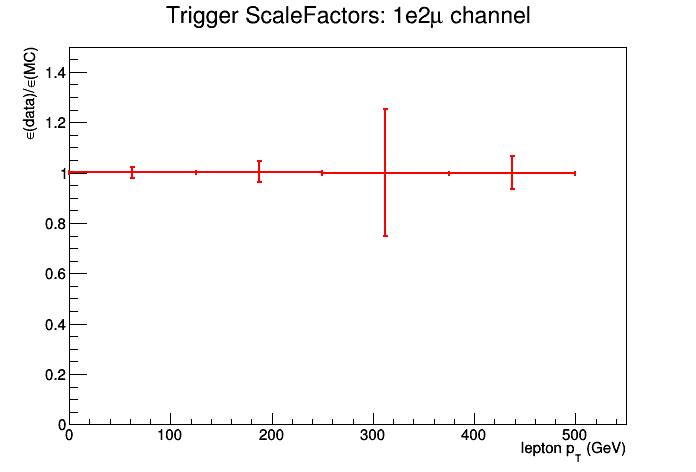
\includegraphics[width=0.48\textwidth]{Figures/trigger/Intext/SF_trigger_1e2muhistPt.png}
%	%		\label{image:SF_trigger_1e2muhistPt.png}
%	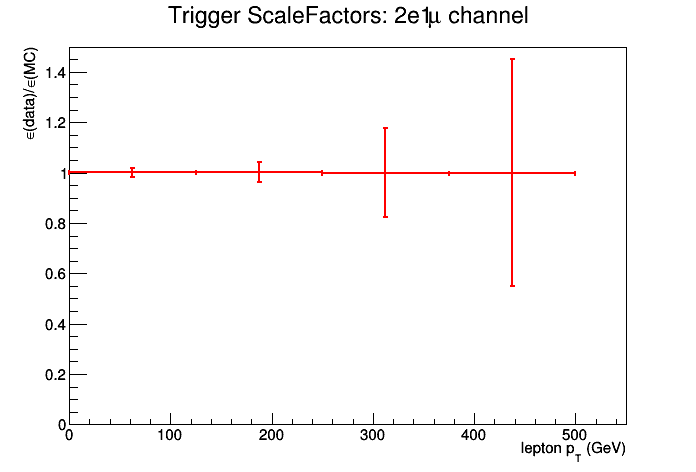
\includegraphics[width=0.48\textwidth]{Figures/trigger/Intext/SF_trigger_2e1muhistPt.png}
%	%		\label{image:SF_trigger_2e1muhistPt.png}
%	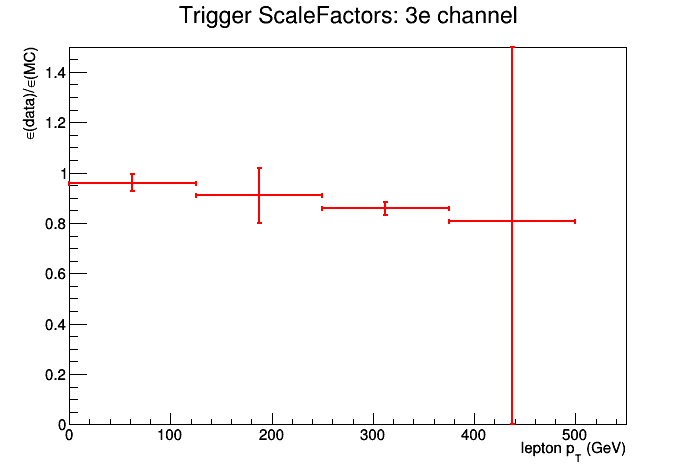
\includegraphics[width=0.48\textwidth]{Figures/trigger/Intext/SF_trigger_3ehistPt.png}
%	%		\label{image:SF_trigger_3ehistPt.png}
%	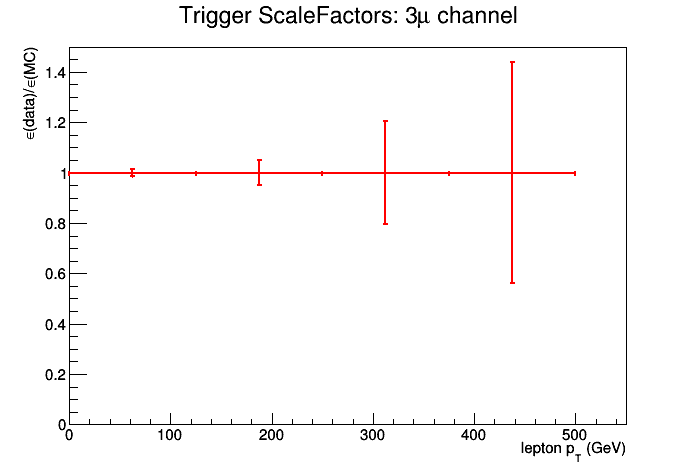
\includegraphics[width=0.48\textwidth]{Figures/trigger/Intext/SF_trigger_3muhistPt.png}
%	%		\label{image:SF_trigger_3muhistPt.png}
%	
%	\caption{The trigger scale factors measured as a function of lepton \pt, using the dataset collected by \Etmis\ triggers and \WZ\ simulation, after a 3 lepton and jets selection, in the Z mass window. All corrections to simulation are applied. Left, upper: 1e2$\mu$ channel. Right, upper: 2e1$\mu$ channel. Left, lower: 3e channel. Right, lower: 3$\mu$ channel}
%	\label{image:FigurestriggerIntext}
%\end{figure}
As can be seen from Appendix \ref{app:trig}, the trigger efficiencies are measured to be nearly 100\% for both simulation and data. The results are dominated by statistics and assigning a large uncertainty to the trigger efficiency based on the dataset collected by \Etmis\ triggers would be over conservative. A one percent uncertainty on the trigger selection for the \eemu\ and \mumumu\ final states, and 5\% for the \eee\ and \emumu\ final states, following the approach of \cite{Sirunyan:2017kkr}, while no scale factors will be applied on simulation as they are close to unity. Control plots are made in the dilepton region to validate all corrections applied to simulation and can be found in \Sec{sec:controldilep}.

\subsection{Corrections}
\label{sec:controldilep}

\label{sec:corrections}
The datasets are processed using the CMSSW 80X\_0\_26\_patch1 release, with the conditions and calibrations as defined in the global tags: 80X\_dataRun2\_2016SeptRepro\_v7 for data and 80X\_mcRun2\_asymptotic\_2016\_TrancheIV\_v8 for simulation. Mismatches have been observed between data and simulation and have to be corrected for. 

\subsection*{Pile up reweighting}
In data, the number of interactions per bunch crossing (pile up) is calculated with a minimum bias cross section of 69.2 mb. The number of simulated pile up events is then reweighed to match the expected number of pile up events in data. Pile up reweighting manifests itself as an altered shape of the number of reconstructed primary vertices as can be seen in Figure \ref{fig:nbvertices}.
%
%\begin{figure}[h]
%	\centering	
%	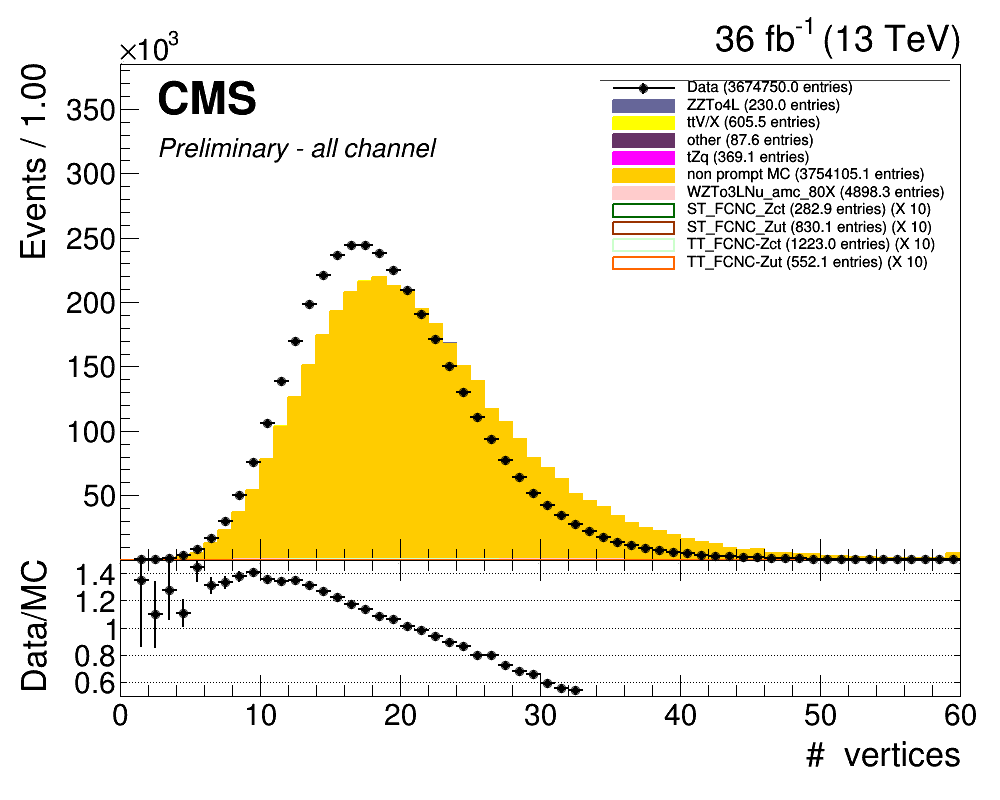
\includegraphics[width=0.45\textwidth]{Figures/Reweighing/pileup/2lepcontrol_afterAtLeast1Jet_afterZWindow_NbOfVertices_all_Stack_before}
%	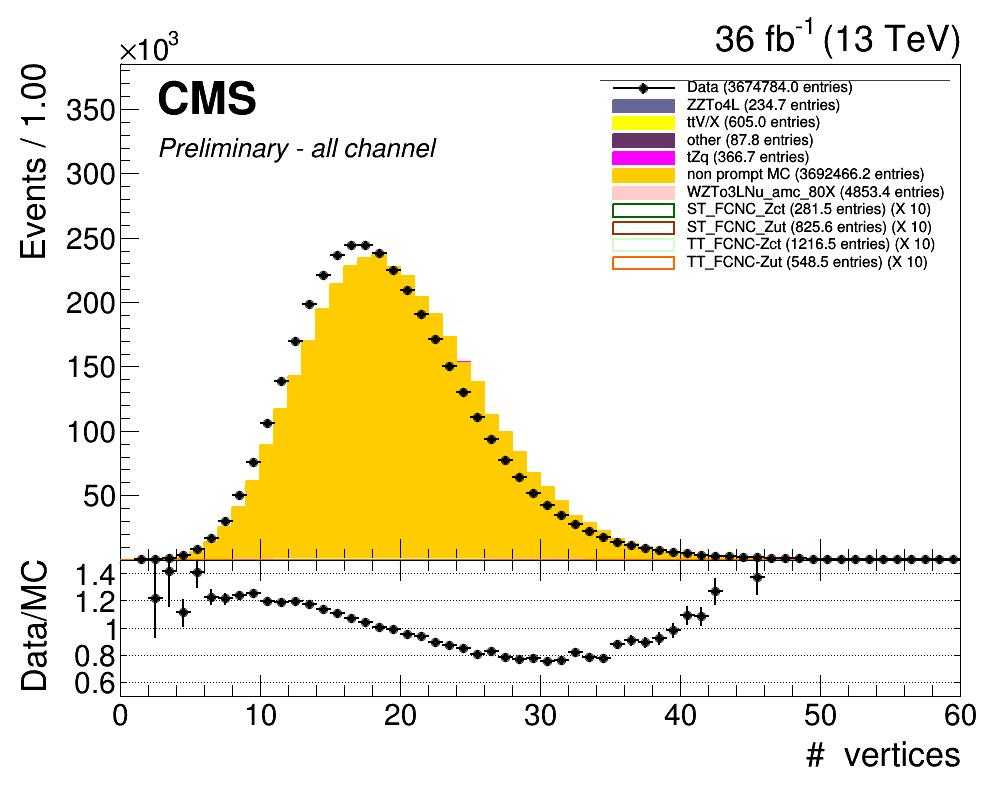
\includegraphics[width=0.45\textwidth]{Figures/Reweighing/pileup/2lepcontrol_afterAtLeast1Jet_afterZWindow_NbOfVertices_all_Stack}
%	\caption{The number of primary vertices before (left) and after (right) pile up reweighting. After a 2 lepton plus jets selection, in the \Z\ mass window.}
%	\label{fig:nbvertices}
%\end{figure}

Note that Figure \ref{fig:nbvertices} indicates that even after pile up reweighting, the primary vertex multiplicity is not well described by simulation. This is a known effect, and using  a minimum bias cross section of 62 or 63 mb was found in other analysis to better describe the data. However, the b tagging scale factors are only provided for the 69.2 mb, and thus this value is used for consistency.


\subsection*{Lepton scale factors}
The efficiency to select leptons is different in simulation ($\epsilon_{\mathrm{MC}}$) compared to the data ($\epsilon_{\mathrm{data}}$) . This is corrected for by applying lepton scale factors (SF) to the simulation that are defined as
\begin{equation}
SF = \frac{\epsilon_{\mathrm{data}}}{\epsilon_{\mathrm{MC}}}. 
\end{equation}
These scale factors are measured for the identification, isolation and trigger efficiencies of the objects as a function of \pt\ and $\eta$. For the muons, an additional tracking efficiency scale factor is applied. Multiplying these scale factors for each lepton provides an overall efficiency:
\begin{equation}
SF^{\mu}_{\mathrm{global}} = \prod \limits_{\mathrm{i}}^{\# \mu}  SF^{\mu}_{\mathrm{ID}}(\pt,\eta) SF^{\mu}_{\mathrm{Iso.}}(\pt,\eta) SF^{\mu}_{\mathrm{Trig.}}(\pt,\eta) SF^{\mu}_{track}(\pt,\eta),
\end{equation}
\begin{equation}
SF^{\mathrm{e}}_{\mathrm{global}} = \prod \limits_{\mathrm{i}}^{\# e}  SF^{\mathrm{e}}_{\mathrm{ID}}(\pt,\eta) SF^{\mathrm{e}}_{\mathrm{Iso.}}(\pt,\eta) SF^{\mathrm{e}}_{\mathrm{Trig.}}(\pt,\eta) .
\end{equation}
The identification and isolation efficiencies are provided by the Muon POG \cite{MUO} and EGM POG \cite{EGM}. The effect of the scale factors can be found in Figure \ref{fig:elSF} and \ref{fig:muSF}. The trigger efficiencies are estimated in Section \ref{sec:triggereff}.

%\begin{figure}[h]
%	\centering
%	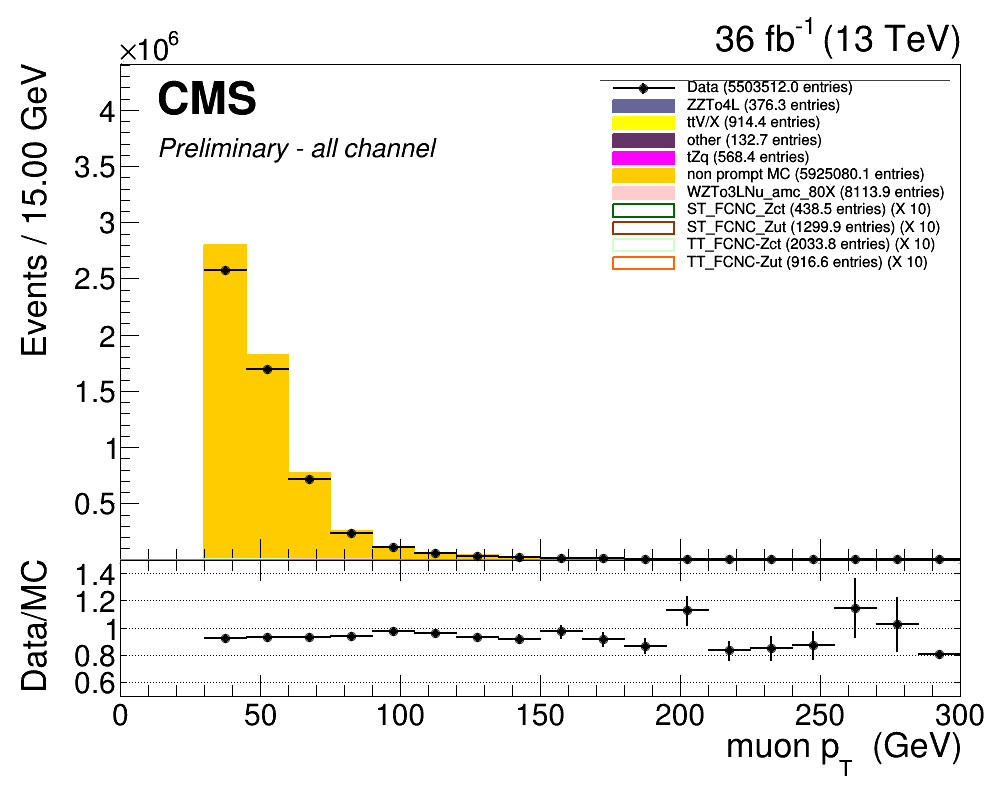
\includegraphics[width=0.45\textwidth]{Figures/Reweighing/muon/2lepcontrol_afterAtLeast1Jet_afterZWindow_MuPt_all_Stack_before}
%	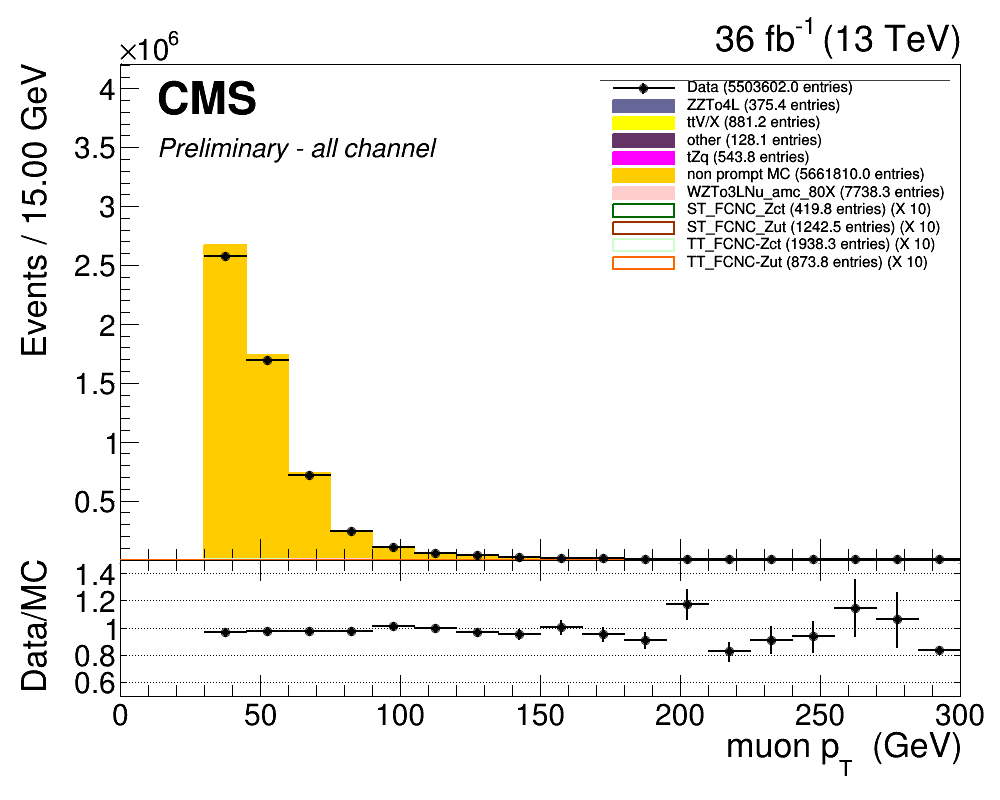
\includegraphics[width=0.45\textwidth]{Figures/Reweighing/muon/2lepcontrol_afterAtLeast1Jet_afterZWindow_MuPt_all_Stack_after}
%	\caption{The \pt\ of the muons before (left) and after (right) muon scale factors. After a 2 lepton plus jets selection, in the \Z\ mass window. Both after the Rochester correction.}
%	\label{fig:muSF}
%\end{figure}
%\begin{figure}[h]
%	\centering
%	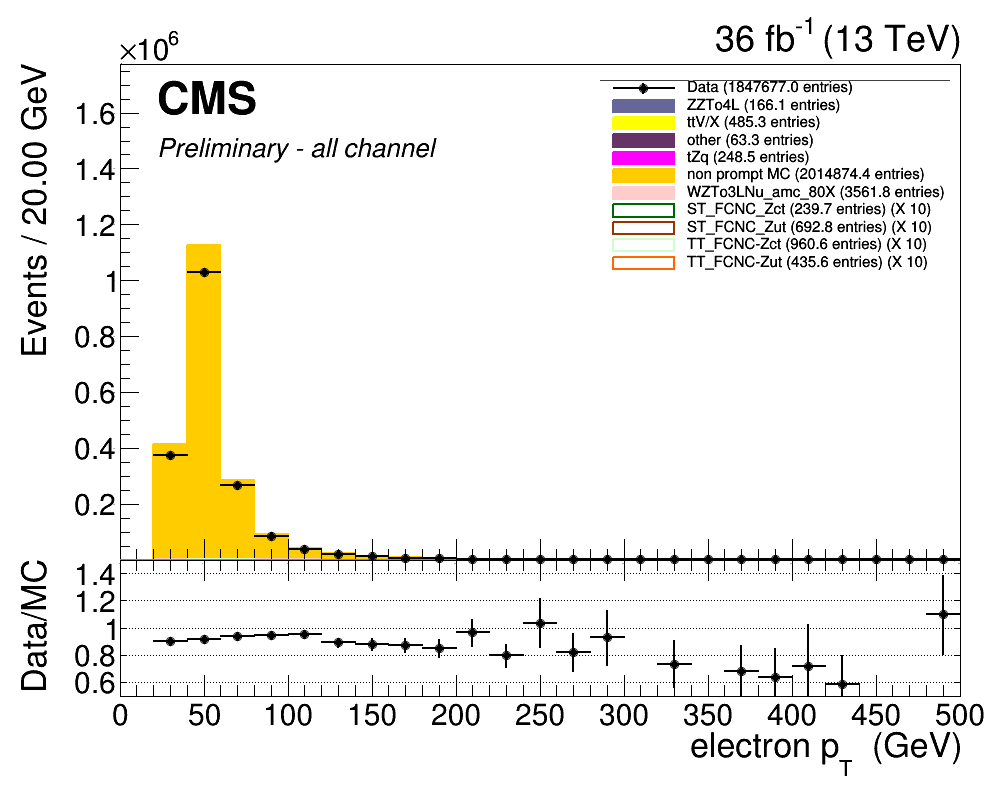
\includegraphics[width=0.45\textwidth]{Figures/Reweighing/electron/2lepcontrol_afterAtLeast1Jet_afterZWindow_ElPt_all_Stack_before}
%	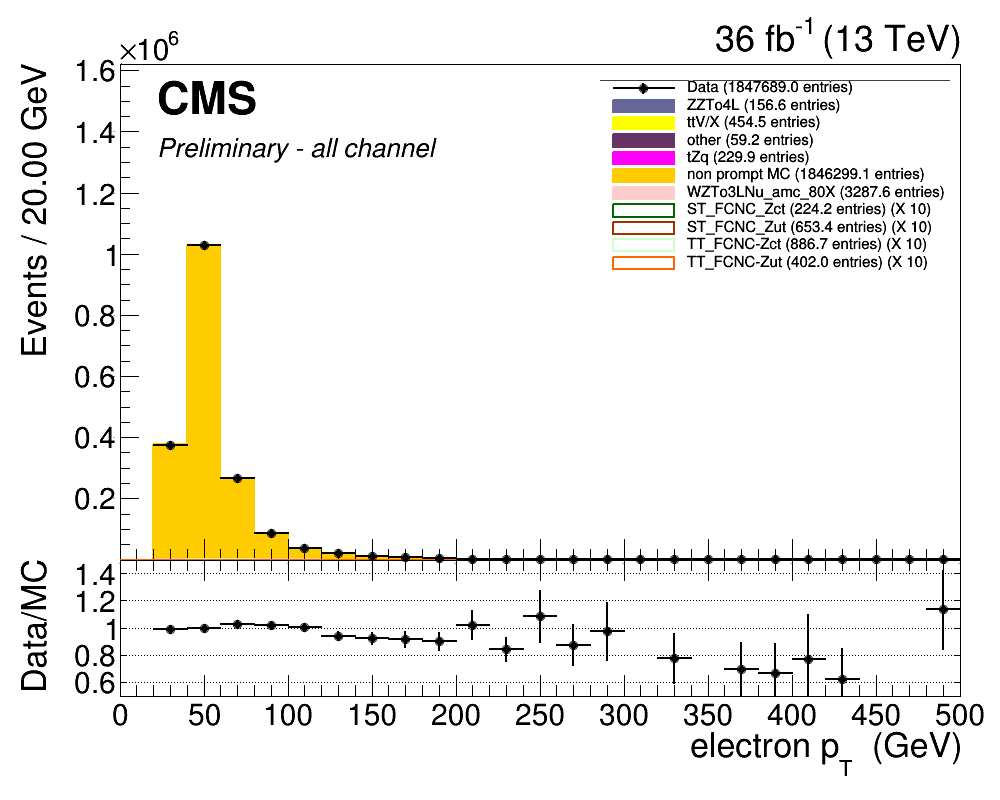
\includegraphics[width=0.45\textwidth]{Figures/Reweighing/electron/2lepcontrol_afterAtLeast1Jet_afterZWindow_ElPt_all_Stack_after}
%	\caption{The \pt\ of the electrons before (left) and after (right) electron scale factors. After a 2 lepton plus jets selection, in the \Z\ mass window. Both after energy scale corrections and smearing.}
%	\label{fig:elSF}
%\end{figure}

Additionally, corrections are made for the energy resolution of the leptons. For the electrons, energy smearing and regression is applied \cite{smearing}. The energy regression uses the detector information to correct the electron energy in order to have the best energy resolution by correcting local energy containment, material effects, etc.. The energy scale and smearing is done in order to bring the data energy scale to simulation level. It smears the simulation energies to have identical energy resolution in simulation and data. For the muons, the \pt\ is corrected using the Rochester method \cite{roch,roch2}. This correction removes the bias of the muon \pt\ from any detector misalignment or any possible error of the magnetic field.
The effect of the Rochester correction can be found in Figure \ref{fig:roch}.
%
%\begin{figure}[h]
%	\centering	
%	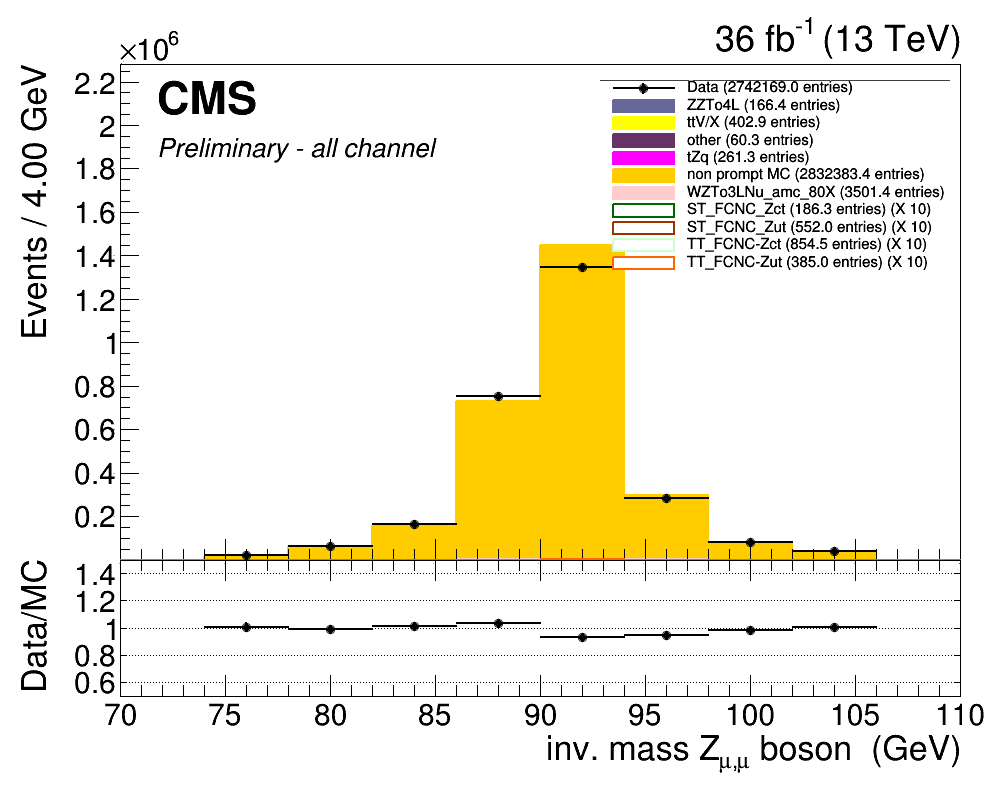
\includegraphics[width=0.45\textwidth]{Figures/Reweighing/rochester/2lepcontrol_afterAtLeast1Jet_afterZWindow_ZbosonMassMu_all_Stack_before}
%	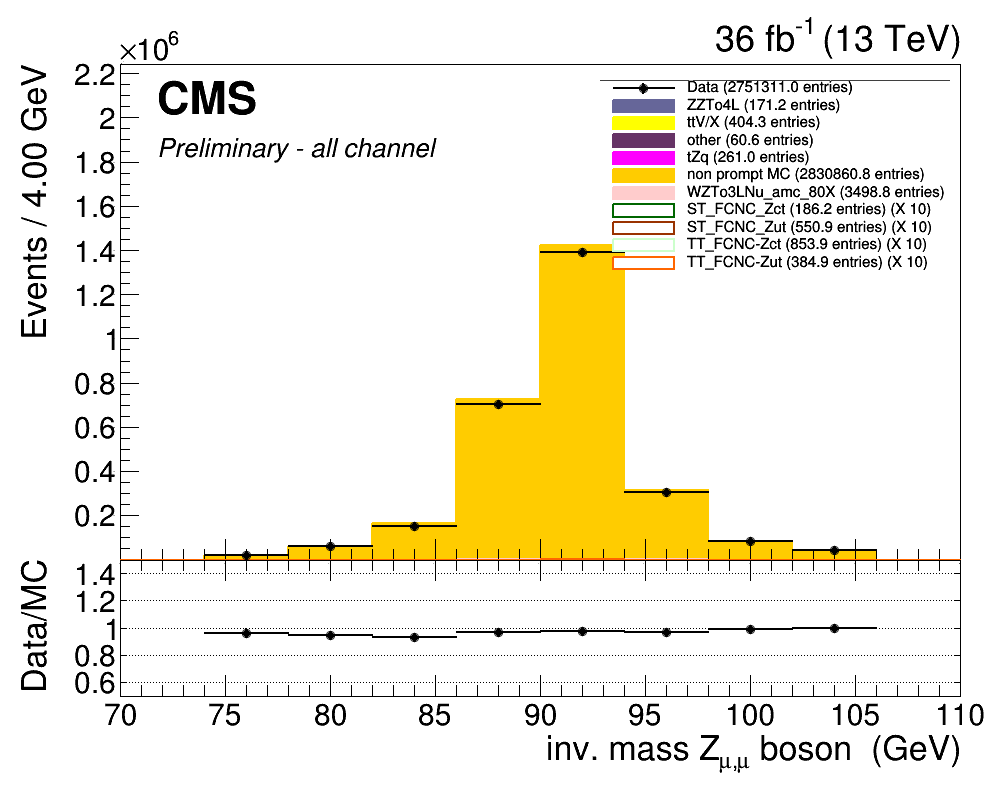
\includegraphics[width=0.45\textwidth]{Figures/Reweighing/rochester/2lepcontrol_afterAtLeast1Jet_afterZWindow_ZbosonMassMu_all_Stack_after}
%	
%	\caption{The mass of the \Z\ boson consisting of the muons before (left) and after (right) the rochester correction. After a 2 lepton plus jets selection, in the \Z\ mass window.}
%	\label{fig:roch}
%\end{figure}

\clearpage
\subsection*{CSVv2 shape correction}
In order to make the shape of the CSVv2 b-tagging discriminant in simulation agree with data,  jet-by-jet based scale factors are applied. The scale factors are provided by the BTV POG \cite{btag} and are a function of the \pt, $\eta$ and CSVv2 value of the jet.  The effect of these scale factors can be found in Figure \ref{fig:bSF}.


%\begin{figure}[h]
%	\centering
%	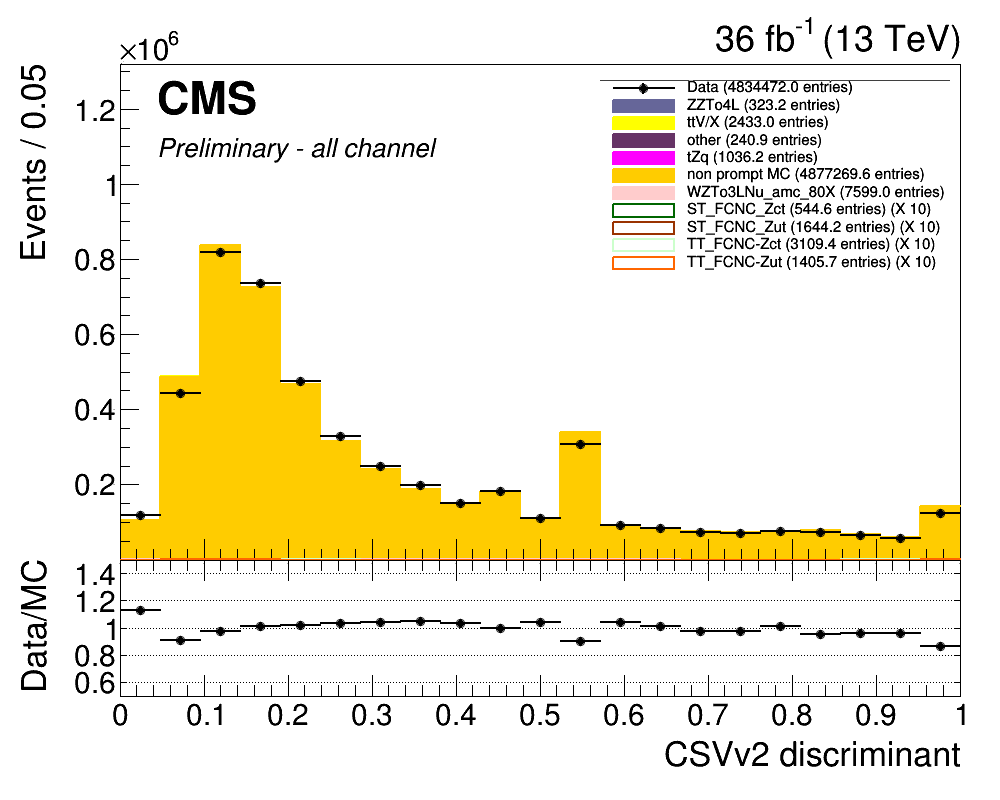
\includegraphics[width=0.45\textwidth]{Figures/Reweighing/bdis/2lepcontrol_afterAtLeast1Jet_afterZWindow_bdisc_all_Stack_before}
%	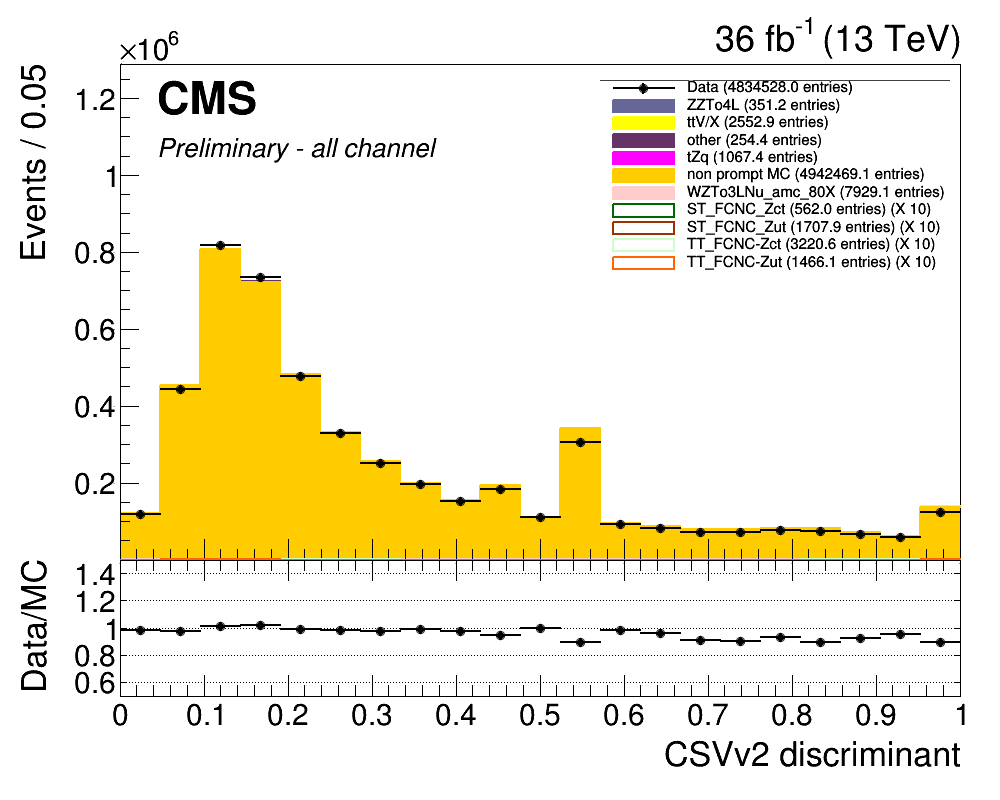
\includegraphics[width=0.45\textwidth]{Figures/Reweighing/bdis/2lepcontrol_afterAtLeast1Jet_afterZWindow_bdisc_all_Stack_after}	
%	\caption{The CSVv2 discriminant of the jets before (left) and after (right) b-tag scale factors. After a 2 lepton plus jets selection, in the \Z\ mass window.}
%	\label{fig:bSF}
%\end{figure}

\subsection*{Jet energy}
\label{sec:jer}
The jet energy in data and simulation is corrected by the measured energy response of the detector. This provides $p_T$- $\eta$ dependent scale factors and are directly taken from the frontier condition database using the global tag Summer16\_23Sep2016V4.
Additionally, the jet \pt\ resolution is corrected by the scaling method described in \cite{jetsmear}, where the jet \pt\ is rescaled by
\begin{equation}
c_{\mathrm{JER}} = 1 + (s_{\mathrm{JER}}-1)\frac{\pt -\pt^{ptcl}}{\pt}.
\end{equation}
With \pt\ the reconstructed transverse momentum, \pt$^{ptcl}$ the transverse momentum of the corresponding jet clustered from generator level particles, and $s_{\mathrm{JER}}$ the resolution scale factor. The resolution scale factor is measured in $\eta$ bins and given in Table \ref{tab:JER}. The effect of the jet energy corrections can be found in Figure \ref{fig:jesSF} and \ref{fig:jerSF}.



%
%\begin{figure}[h]
%	\centering
%	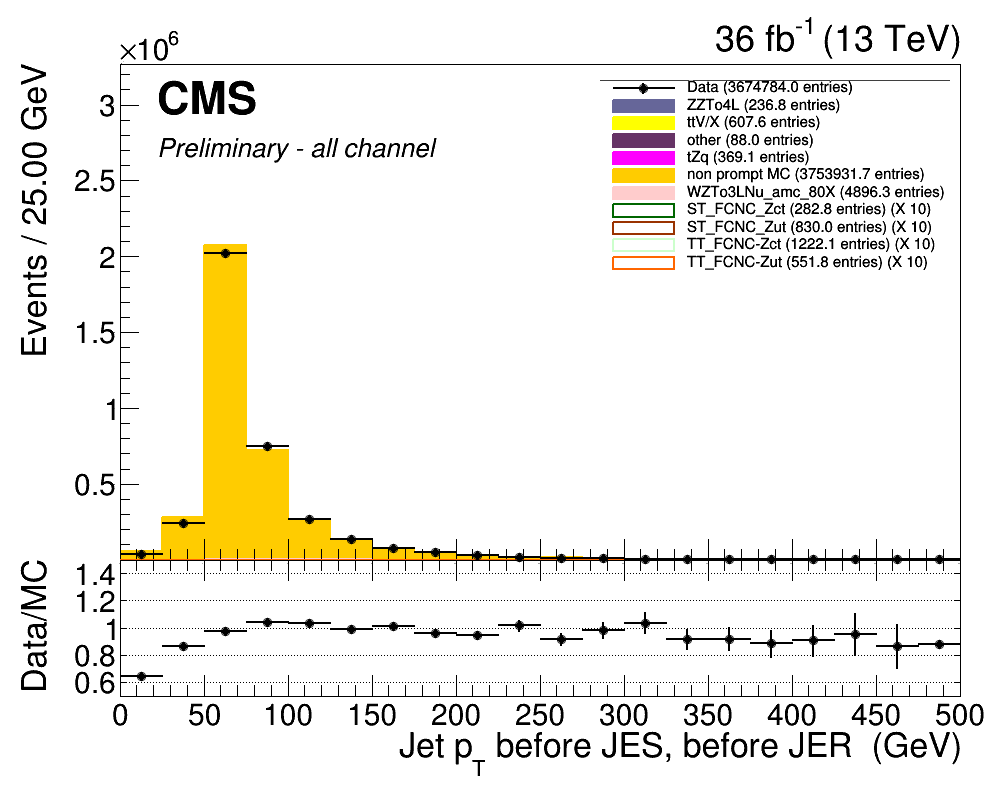
\includegraphics[width=0.45\textwidth]{Figures/Reweighing/JEC/2lepcontrol_afterAtLeast1Jet_afterZWindow_JetPt_bfJES_all_Stack}
%	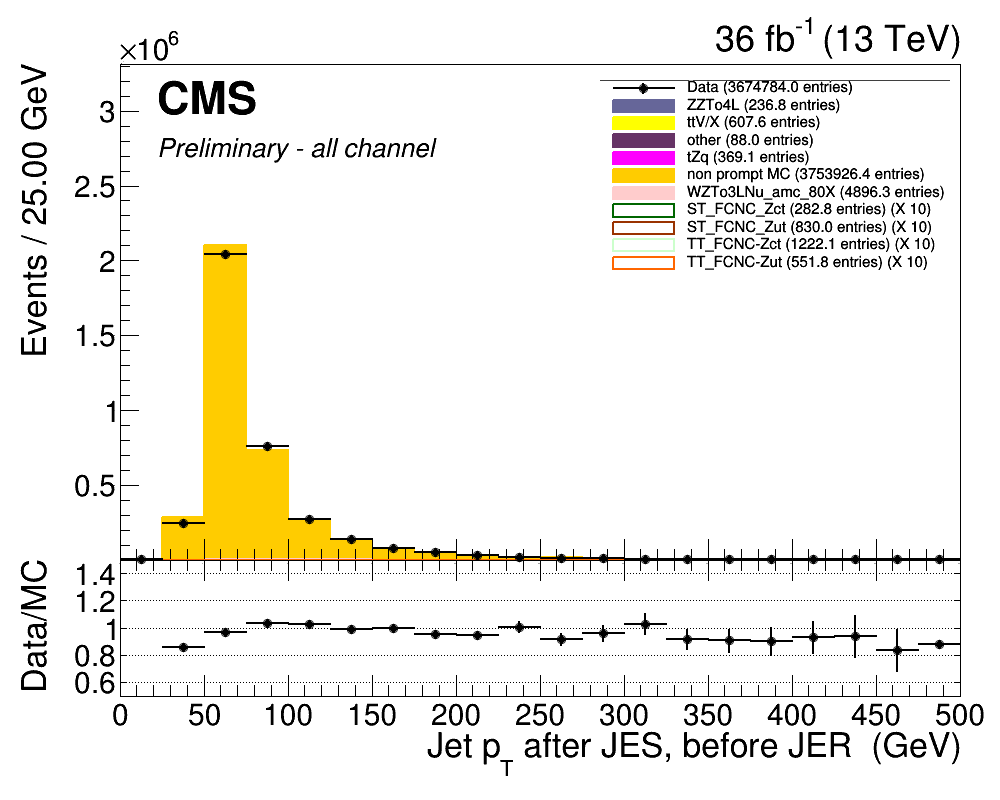
\includegraphics[width=0.45\textwidth]{Figures/Reweighing/JEC/2lepcontrol_afterAtLeast1Jet_afterZWindow_JetPt_afJES_all_Stack}
%	\caption{The \pt\ of the jets before (left) and after (right) jet energy scale corrections. After a 2 lepton plus jets selection, in the \Z\ mass window.}
%	\label{fig:jesSF}
%\end{figure}

%\begin{figure}[h]
%	\centering
%	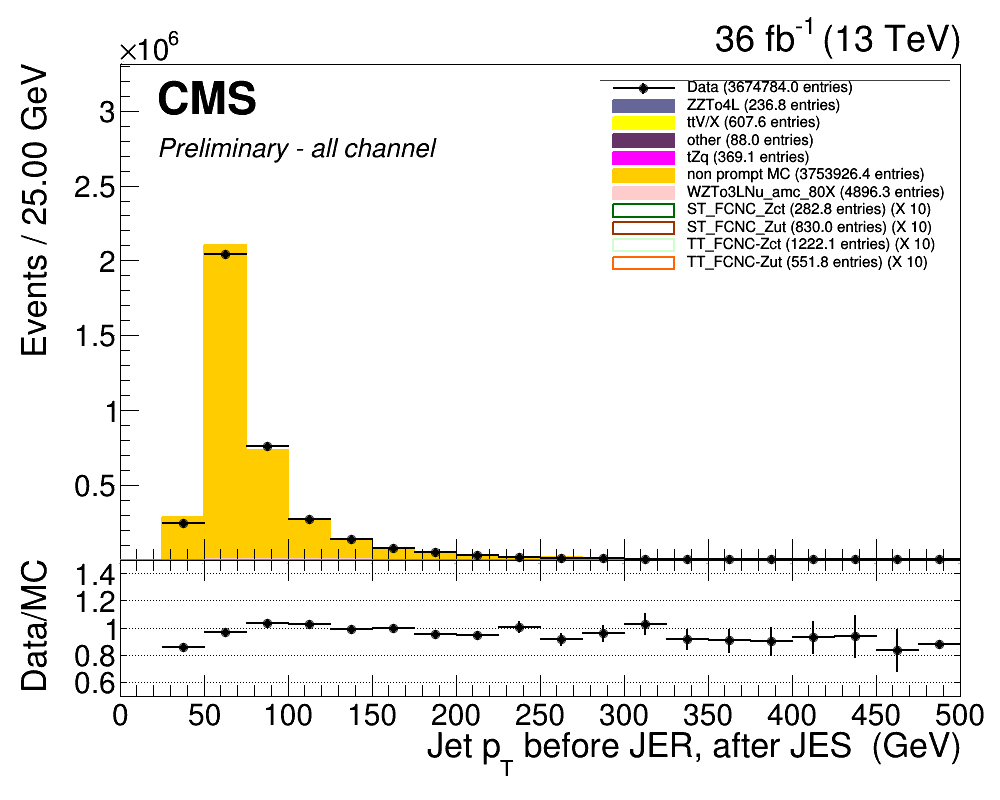
\includegraphics[width=0.45\textwidth]{Figures/Reweighing/JER/2lepcontrol_afterAtLeast1Jet_afterZWindow_JetPt_bfJER_all_Stack}
%	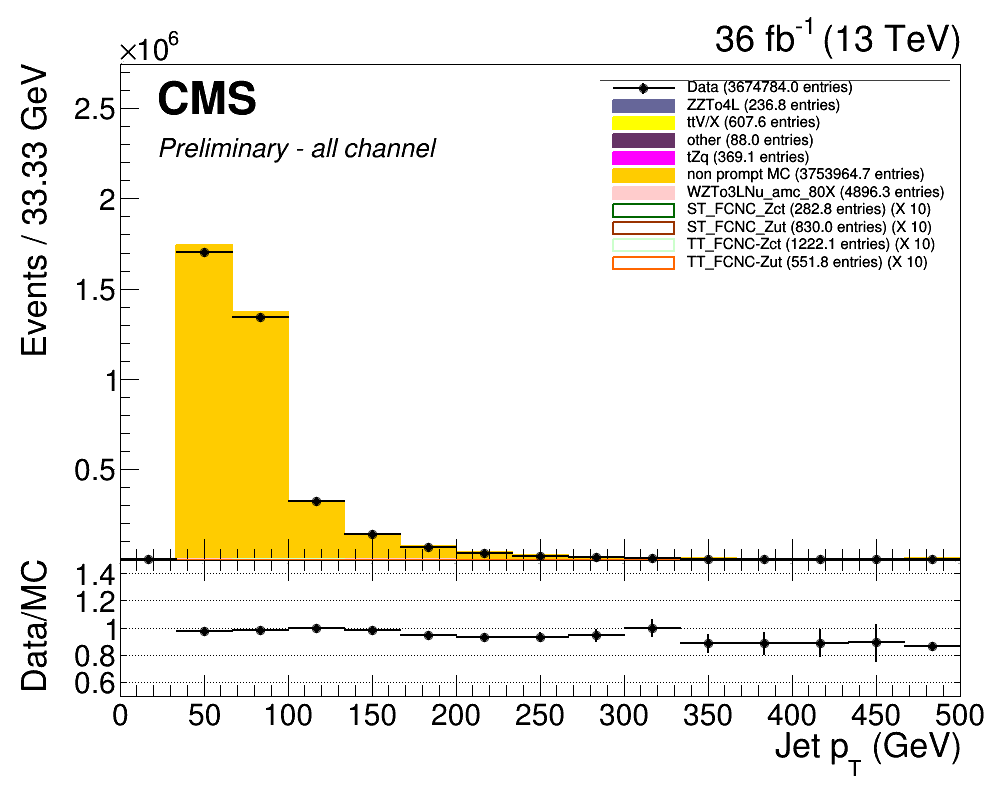
\includegraphics[width=0.45\textwidth]{Figures/Reweighing/JER/2lepcontrol_afterAtLeast1Jet_afterZWindow_JetPt_afJER_all_Stack}
%	\caption{The \pt\ of the jets before (left) and after (right) jet energy resolution smearing. After a 2 lepton plus jets selection, in the \Z\ mass window.}
%	\label{fig:jerSF}
%\end{figure}


\subsection*{Missing transverse energy}
The energy scale and resolution corrections applied to the jets are propagated back to the  missing transverse energy (smeared Type I correction). This rebalances the transverse net momentum of the event and improves the missing transverse energy resolution itself.

\section{Analysis Strategy}
\label{sec:selection}


The analysis strategy uses five statistically independent regions to extract limits using a likelihood fit of various observables. Two signal regions, the \tZ\ (\STSR) and \tZq\ (\TTSR) signal region, are constructed using the jet multiplicity,  focussed on each signal signature (see Tab. \ref{tab:Regions}).  In order to constrain the rate of \WZ+jet events as well as that of nonprompt lepton backgrounds three control regions are defined. The \WZ\ control region (\WZCR) focusses on nonprompt leptons originating from \DY\ and simultaneously constrains the \WZ+jets background rate. The nonprompt lepton backgrounds coming from \ttbar, are constrained by two control regions, \TTCR\ and \STCR, one for each signal region (\TTSR\ and \STSR).  In the \STSR\ and \TTSR\, multivariate discriminants based on Boosted Decision Trees (BDT) are used to respectively discriminate \FCNC\ \tZ\ and \FCNC\ \tZq\ from backgrounds. In the \WZCR\ a  discriminating variable between the two backgrounds, \WZ+jets and nonprompt leptons, is used. In \TTCR\ and \STCR\, the dominating process is \ttbar\, and its rate is estimated by subtracting all other background predictions from data. A simultaneous global fit is performed taking into account each region (\STSR, \TTSR, \WZCR, \TTCR\ and \STCR) for the four different leptonic channels. 

\section{Data driven background simulation}
\label{sec:NPL}

The MC samples are used to model the backgrounds as well as for training the boosted decision trees
for signal to background separation. One of the most important background consist of events with nonprompt leptons. These are mostly instrumental background and are therefore very difficult to model. The nonprompt lepton background is estimated from data for both its shape and its normalisation. 

The nonprompt lepton sources are 
\begin{itemize}
	\item hadronic objects wrongly reconstructed as leptons, 
	\item real leptons coming from the semi leptonic decay of a \b\ or \c\ hadron,
	\item real leptons coming from the conversion of photons, 
\end{itemize}
that pass the identification and isolation requirements. The dominant source of these nonprompt leptons depend on the flavour of the lepton and therefore the events with a nonprompt muon are treated differently than those with a nonprompt electron. For muons, the dominant source is the semi leptonic decay of heavy flavour hadrons. For electrons, the dominant sources are hadrons and photon conversions. 

The backgrounds causing nonprompt lepton contributions are mostly Drell--Yan (\DY) and \ttbar\ dilepton processes, and in a smaller amount \WW\ and \tWZ. All of these backgrounds contain two real leptons and one nonprompt lepton. Due to the fact that the probability for a lepton to be a nonprompt lepton is small, backgrounds containing two or more nonprompt leptons are neglected. The assumption is made that for DY the two leptons compatible with a \PZ\ boson decay are the real leptons, and the additional lepton is coming from a nonprompt lepton source, while for \ttbar\ the nonprompt lepton is associated to the Z boson. 

The nonprompt lepton sample is constructed from data by requiring exactly three leptons, from which two are considered real, isolated leptons and the third is a nonprompt lepton. This nonprompt lepton is created by loosening its identification and inverting its isolation criteria. The full requirements on the (nonprompt) leptons are given in  \tab{tab:nonpromptel} and \tab{tab:nonpromptmu}.  For nonprompt electrons, a large fraction is coming from misidentified photons. These are removed by applying a tighter cut on the $1/E-1/p$ variable, and by limiting the isolation values to be smaller than one. 
\begin{table}[htbp]
	\centering
	
	\caption{Non prompt electron requirements used in this analysis. The requirements are set in the barrel ($|\eta_{supercluster}| \leq 1.479$)
		and the end caps ($|\eta_{supercluster}| > 1.479$). }
	\begin{tabular}{ccc}
		\toprule
		& \multicolumn{1}{c|}{$|\eta_{supercluster}| \leq 1.479$ } & \multicolumn{1}{c}{$|\eta_{supercluster}| > 1.479$ } \\
		\midrule
		$\sigma_{\eta \eta}$ & $<$ 0.011 & $<$ 0.0314 \\ 
		
		$|\Delta\eta_{\mathrm{in}}|$ & $<$ 0.00477& $<$ 0.00868\\ 
		
		$|\Delta\phi_{\mathrm{in}}|$ & $<$ 0.222 &  $<$ 0.212 \\ 
		 
		H/E & $<$ 0.298& $<$ 0.101 \\ 
		
		relative isolation & $\geq$ 0.0588 \&\& $<$ 1 &  $\geq$ 0.0571 \&\& $<$ 1\\ 
	
		$|1/E-1/p|$ & $<$ 0.0129 \GeVinv & $<$ 0.0129 \GeVinv \\ 
		
		expected missing inner hits & $\leq $ 1 &  $\leq $ 1\\ 
	
		pass conversion veto & Y & Y \\ 
	
		\pt &$>$ 35 \GeV & $>$ 35 \GeV \\
		\bottomrule
	\end{tabular} 
	\label{tab:nonpromptel}
\end{table}

\begin{table}[htbp]
	\centering
	\caption{Non prompt muon requirements used in the analysis. }
	
	\begin{tabular}{cc}
		\toprule
		& modified Loose Muon WP \\ 
		\midrule 
		Global muon or Tracker Muon & Both  \\ 
		
		Particle Flow muon & Y  \\ 
		
		$\chi^2/ndof$ of global muon track fit & N/A \\  
		
		Nb. of hit muon chambers & N/A \\ 
		 
		Nb. of muon stations contained in the segment & N/A   \\ 
		
		Size of the transverse impact parameter  of the track wrt. PV & N/A  \\ 
		 
		Longitudinal distance wrt. PV & N/A \\ 
		
		Nb. of pixel hits & N/A \\ 
		
		Nb. of tracker layers with hits & N/A  \\ 
		
		Relative Isolation & $\geq$ 0.15 \\
		
		\pt &$>$ 30 \GeV  \\
		\bottomrule
	\end{tabular} 
	
	\label{tab:nonpromptmu}
\end{table}


The nonprompt leptons samples are defined in a given control region and are used to describe their contribution in the other regions. 

\newpage
\section{Regions and channels}
\label{sec:regions}
The regions are defined as in Table \ref{tab:Regions} after a common selection of
\begin{itemize}
	\item exactly 3 leptons containing one opposite sign, same flavour pair,
	\item at least 1 jet and at the most 3 jets,
	\item the transverse mass of the \PW\ boson to be maximal 300 \GeV,
\end{itemize}
The cut on the transverse mass of the \PW\ boson is done to remove events that are passing the events cleaning although they shouldn't.
The transverse mass $\mtw$ is reconstructed using
\begin{equation}
\mtw = \sqrt{(\pt(l_{\W}) + \pt(\nu_{\W}) ) ^2 - (p_{\mathrm{x}}(l_{\W}) + p_{\mathrm{x}}(\nu_{\W}))^2  - (p_{\mathrm{y}}(l_{\W}) + p_{\mathrm{y}}(\nu_{\W}))^2    }
\end{equation}

\begin{table}[htbp]
	\centering
	\caption{The statistically independent regions used in the analysis.}
	\begin{tabular}{c|c|c|c|c|c}
		\hline 
		& \WZ  & \tZ  & \tZq  & \tZ  & \tZq\\ 
		&  control region &  signal region & signal region &  control region & control region\\ 
		& (\WZCR)& (\STSR)  & (\TTSR) & (\STCR) & (\TTCR) \\ 
		\hline 
		Number of jets & $\geqslant 1$, $\leq 3$ & 1 & $\geqslant 2$, $\leq 3$  & 1 & $\geqslant 2$, $\leq 3$\\ 
		\hline 
		Number of b jets & 0 & 1 & $\geqslant 1$  & 1 & $\geqslant 1$ \\ 
		\hline 
		$|M(\PZ_{\mathrm{reco}}) - \mZ|$ & Yes & Yes & Yes & No & No \\
		$< 7.5$ \GeV &  &  &  &  &  \\
		\hline  
	\end{tabular} 
	\label{tab:Regions}
\end{table}

Additional leptons are vetoed in order to reduce the contamination of backgrounds with four or more leptons in the final state, e.g. \ZZ, \ttZ, and \ttH. The most important backgrounds are the ones that contain three prompt leptons in the final state. These are mainly \WZ +jets, \ttZ and SM \tZq. For these backgrounds, the three lepton topology is identical to the \FCNC\ signal: two opposite sign leptons of the same flavour decaying from the \PZ\ boson, and a third additional, high \pt\ lepton coming from the \PW\ boson decay.

For the FCNC \tZ\ final state, one b jet coming from the SM top decay is expected. For the FCNC \tZq, an additional light jet is expected. In the \ttZ\ final state, two b jets are present in the final state. However, due to inefficiencies of the b-tagging algorithm, one of the two b jets may be identified as a light quark jet, giving the same final state as the FCNC \tZq\ final state. For the \WZ+jets final states, one of the b jets produced by gluon splitting can be b-tagged or light flavour jets coming from the \WZ+jets production can be mis-tagged as b jets. The SM \tZq\ final state expects the same signal as FCNC \tZq.
% (\FIXME recheck all leading bkg in STSR). 

The \NPL\ lepton distribution gives a significant background contribution. This background is coming mainly from \DY\ and \ttbar\ processes (in a less significant way, also \WW\ and \tWZ\ contributes), which have very high cross sections and causes a large number of nonprompt  background events, compared to signal.

In order to reduce the large uncertainties in backgrounds, five independent regions are used as defined in Table  \ref{tab:Regions}. 


\subsection{WZ control region}
In this region, a fit is performed on the transverse mass of the \PW\ boson, in order to estimate the nonprompt  lepton yield coming from \DY\ and the \WZ+jets backgrounds. 

A transfer factor has to be used to account for going from a region with 0 b jets to a region with exactly one jet, or at least one jets. For this the probability of tagging at least one jet with the CSVv2 loose working point is used to calculate the expected number of events, Nb, after b tagging: 
\begin{align}
	Nb = \frac{\sum_{events}\text{P(event survives b tag)}}{\text{total nb of events}}
\end{align}
where 
\begin{align}
	\text{P(event survives b tag )} &= 1 - \text{P(event doesn't survive b tag)}\\
	& = 1 - \left(\prod_{b} \text{P(b not tagged)} \prod_{c} \text{P(c not tagged)} \prod_{udsg} \text{P(light not tagged)}\right)\\
	& = 1 - \left(\prod_{b} 0.10 \prod_{c} 0.40 \prod_{udsg} 0.90\right)
\end{align}
with the products going over all b-, c-, and light jets. For this, the jet flavour is taken by means of matching the reconstructed jet to the generated quark based on $\Delta R = \sqrt{\Delta \phi^2 + \Delta \eta^2}$/.  
In order to go to exactly one b jet, this expected number of events is corrected by the fraction of events with exactly  one jet in the \WZCR. The resulting transfer factors are given in Appendix \ref{app:tablestr}. One can see  that the yield of \WZ+jets events in the signal region estimated using the above described transfer factor and the yield calculated with simulated events are in agreement. 

\subsection{\TTCR\ and \STCR}
The \TTCR\ and \STCR have the same selection criteria as \TTSR\ and \STSR\, but are outside the \PZ\ mass window (sidebands): 
\begin{equation}
7.5 \: GeV < |M(Z_{reco}) - M(Z)| < 30 \:GeV. 
\end{equation}
where $M(Z_{reco})$ is the reconstructed mass of the \PZ\ boson in the event, and $M(Z)$ the mass of the \PZ\ boson.
These regions are dominated by \ttbar\ (see Appendix \ref{app:tablestr}) and are used to estimate the nonprompt  leptons coming from \ttbar\ in the \STSR\ and \TTSR. Since there aren't enough events entering these regions, no shapes are used in the fit. The distribution of the mass of the Z boson is flat for \ttbar\ events, as shown in Fig. \ref{fig:3lepcontrolafteratleast1jet3lepzbosonmassallnormalized},  and thus the number of expected events, $Ns$, in the signal regions estimated from the number of expected events, $Nc$, in the control region is obtained as
\begin{equation}
Ns = \frac{15}{60-15} Nc.
\end{equation}
The resulting transfer factors are given in Appendix \ref{app:tablestr}. The expected yield in the signal region estimated from the \TTCR\ (\STCR) is in agreement with the yield calculated from simulated events. 


%\begin{figure}[ht]
%	\centering
%	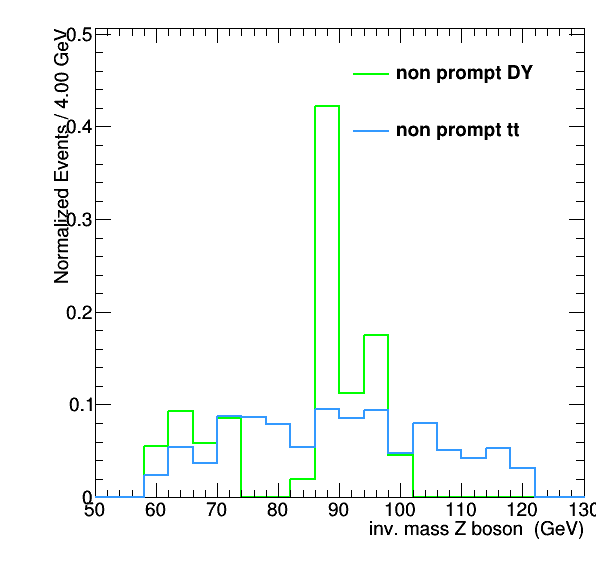
\includegraphics[width=0.47\linewidth]{ZbosonMass/3lepcontrol_afterAtLeast1Jet_3lep__ZbosonMass_all_Normalized}
%	\caption{The normalized distribution for \DY\ and \ttbar\ events before dividing the events in to regions, after $|M(Z_{\mathrm{reco}}) - M(Z)| < 30$ GeV. All leptonic channels combined.}
%	\label{fig:3lepcontrolafteratleast1jet3lepzbosonmassallnormalized}
%\end{figure}

\subsection{\TTSR\ and \STSR}
The \TTSR\ is defined to target top quark pair FCNC (\tZq), while the \STSR\ focusses on single top quark FCNC (\tZ). They have nonprompt  lepton contributions coming from \DY\ and \ttbar\ events. In this region, the data driven nonprompt  lepton template is split into two templates based on the presence of the non isolated lepton in the Z boson: 
\begin{itemize}
	\item Non prompt lepton associated with \PW\ boson is assigned to \DY\ and estimated in the \WZCR.
	\item Non prompt lepton associated with \PZ\ boson is assigned to \ttbar\ and estimated in the \TTCR\ and \STCR.
\end{itemize}
It is shown in Appendix \ref{app:BDTnp}, that these two templates have the same shape within the limited statistics, not assuming any systematic uncertainties. 

